\documentclass[conference]{IEEEtran}
\IEEEoverridecommandlockouts
% The preceding line is only needed to identify funding in the first footnote. If that is unneeded, please comment it out.
\usepackage{cite}
\usepackage{amsmath,amssymb,amsfonts}
\usepackage{algorithmic}
\usepackage{graphicx}
\usepackage{textcomp}
\usepackage{verbatim}
\usepackage{xcolor}
\usepackage{fancyhdr}

\def\BibTeX{{\rm B\kern-.05em{\sc i\kern-.025em b}\kern-.08em
    T\kern-.1667em\lower.7ex\hbox{E}\kern-.125emX}}
\pagestyle{fancy}
\fancyhf{}
\rfoot{Mentor: Prof. Jayprakash Lalchandani}
\begin{document}
\title{Slicing Java Programs\\
%{\footnotesize \textsuperscript{*}Note: Sub-titles are not captured %in Xplore and
%should not be used}
}

\author{\IEEEauthorblockN{1\textsuperscript{st} Rutvik Modi(201701222)}
\IEEEauthorblockA{\textit{Information and Communication Technology} \\
\textit{DAIICT}\\
Gandhinagar, India \\
rutvikmodi1299@gmail.com}
\and
\IEEEauthorblockN{2\textsuperscript{rd} Nirmit Shah(201701044)}
\IEEEauthorblockA{\textit{Information and Communication Technology (CS minor)} \\
\textit{DAIICT}\\
Gandhinagar, India \\
shahnirmit2503@gmail.com}
}

\maketitle

\begin{abstract}
The software  industry is growing very rapidly and the programs written by the developers are quite large having thousands and lacs of lines and hence to analyze the impact of a line of a code and debugging it, in such a large program would be a very tedious task. However, the tedious task can become easier if instead of thousands of lines, consisting of some lines that is of no use in reference to the variable we are analysing. Program Slicing is defined as retrieving statements as a slice of program that may potentially affect the value of the variable that is of interest at a particular time in a program. This project aims at developing a Java dynamic slicer which would support various functionalities of Java language.
\end{abstract}

\section{Introduction}
As mentioned above, program slicing is retrieving instructions that affect a variable of interest at a particular time in the program.There are two types of slicing, the first being static and the other being dynamic. Static slicing does not take user input into consideration while dynamic slicing considers user input in order to compute a program slice. Also, the slicing methods can be implemented by maintaining some kind of dependency graph or by using certain graph-less techniques. We have focused on the graph-based algorithms for dynamic slicing in this project.

Slicing a program is defined in terms of a slicing criterion which includes the following things:
\begin{itemize}
    \item The variable of interest
    \item The line number in the program
    \item User input for the variables in the program
\end{itemize}

Dynamic slicing is more helpful in debugging a variable than static slicing as static slicing includes all the instructions that might not be executed for a particular user input while the dynamic slices only contains executed instructions. Due to this reason, implementing dynamic slicing is a more tedious job and requires additional efforts since apart from the dependencies, one needs to also find the statements that have been executed for a user input.

As Java is one of the primary languages used in the software industry, we chose to implement a dynamic slicer which works for Java programs.

\section{Related Work}
The section describes the research papers that we reviewed which gave us the idea of what program slicing is and different types of algorithms that can be implemented for dynamic slicing a program.

Frank Tip in his research paper\cite{b2} explained about different types of dependencies that needs to be considered while creating a dependency graph. The research paper also discusses the applications of program slicing. 

Hiralal and Joseph in their research paper\cite{b1} explained the idea of dynamic slicing by explaining the idea of PDG and static slicing and proposed different possible implementations of dynamic slicing. The research paper also evaluates the output slices computed via different algorithms and describes the advantages and disadvantages of a particular algorithm. 

Matthew Bridges in his research paper\cite{b3} explained different kind of dependency graphs and also described slicing algorithms for parallel programs. The research paper also presented a graph based technique to handle the functional calls present in a program. 

\section{Basic Constructs}

\subsection{Basic Block}
A basic block in a program is some set of consecutive statements such that there are no multiple entry or exit points. Conditional statements like if-else and loops in standard programming languages can not be a part of basic block since they have multiple exit points. Basic block can consist of a single instruction or may have multiple instructions. For the algorithm, we have considered basic blocks to have only one instruction.
\subsection{Control Flow Graph}
A control flow graph is useful for showing the direction of flow of the program. It is a directed graph whose vertexes are basic blocks and the edges represent control flow between the vertex. The control flow edge represents that there exists at-least one execution path from x to y.
\subsection{Program Dependence Graph}
Program dependence graph(PDG) is a directed graph with nodes as statements and edges as data dependencies and control dependencies. 
\subsection{System Dependence Graph}
System Dependence Graph are different PDGs for different procedures connected with the help of edges and nodes at calling location.

\section{UML Diagrams}
\subsection{User Stories }\label{AA}
\begin{itemize}
    \item As a user, I want a tool to slice a java code so that I can debug a particular variable
    \item As a user, I want a dynamic slicer, so that I can find dependencies of a particular variable
    \item As a user, I want to see a dependency graph, so that I can visualize the slice in a better way
    \item As a user, I want a tool in which I can upload the Java program, so that i
    \item As a user, I want a tool in which I can see the code after uploading, so that I can ensure that I have uploaded correct file
    \end{itemize}

\subsection{Activity Diagram}
    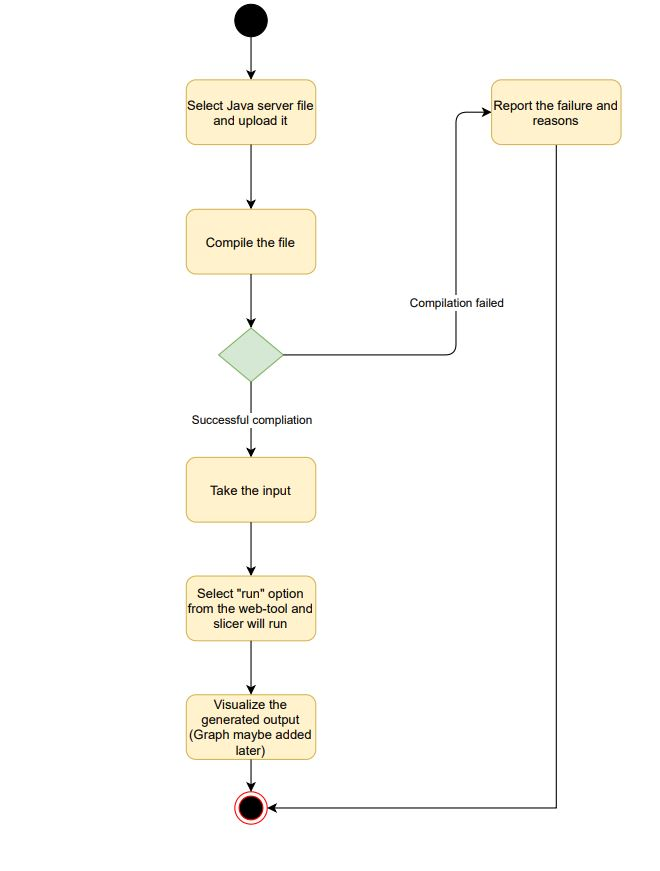
\includegraphics[scale = 0.6]{project1.JPG}
The above figure shows the Activity Diagram representation of the dynamic slicer tool. 
\section{Logic and Implementation}
We can think of this problem as (i) Constructing a dependency graph (ii) Using a graph reachability algorithm on the dependency graph to compute the dynamic slice. Thus, first of all, we need to implement a code parser, then find out the line numbers of the instructions that will actually be executed depending upon the user inputs. Once the dependency graph has been created, the second part is relatively easier to implement.
\subsection{Code Parser}
The most important part of slicers is to implement a code parser that can parse the Java keywords. Now, the role of the parser is to execute source code line-wise and since we want a dynamic slicer, while parsing the code we need to store the line numbers of the instructions or the instructions that have been executed after user inputs the variables. Also, Java being a quite wide-spreaded language, we decided the keywords which we want our slicer to handle. The list of keywords and functionalities that the slicer can successfully handle are as below:
\begin{itemize}
    \item For loop
    \item While loop
\item If else
 \item Try catch block
 \item Return statements
 \item Data Types (int, float, double, string, void, long)
 \item Scanner class
 \item Methods : Public static methods (void and int)
 \item Threading : Basic methods (object.start(), run method, thread.getid())
 \item API calls
 \item Function calls
 \item URL Connection
 \item Connection Request Method
 \item Iterators
 \item Comments
 \item Arithmetic operations
 \item String operations
 \item Assignment operations
\end{itemize}
\subsection{Schematic diagram}
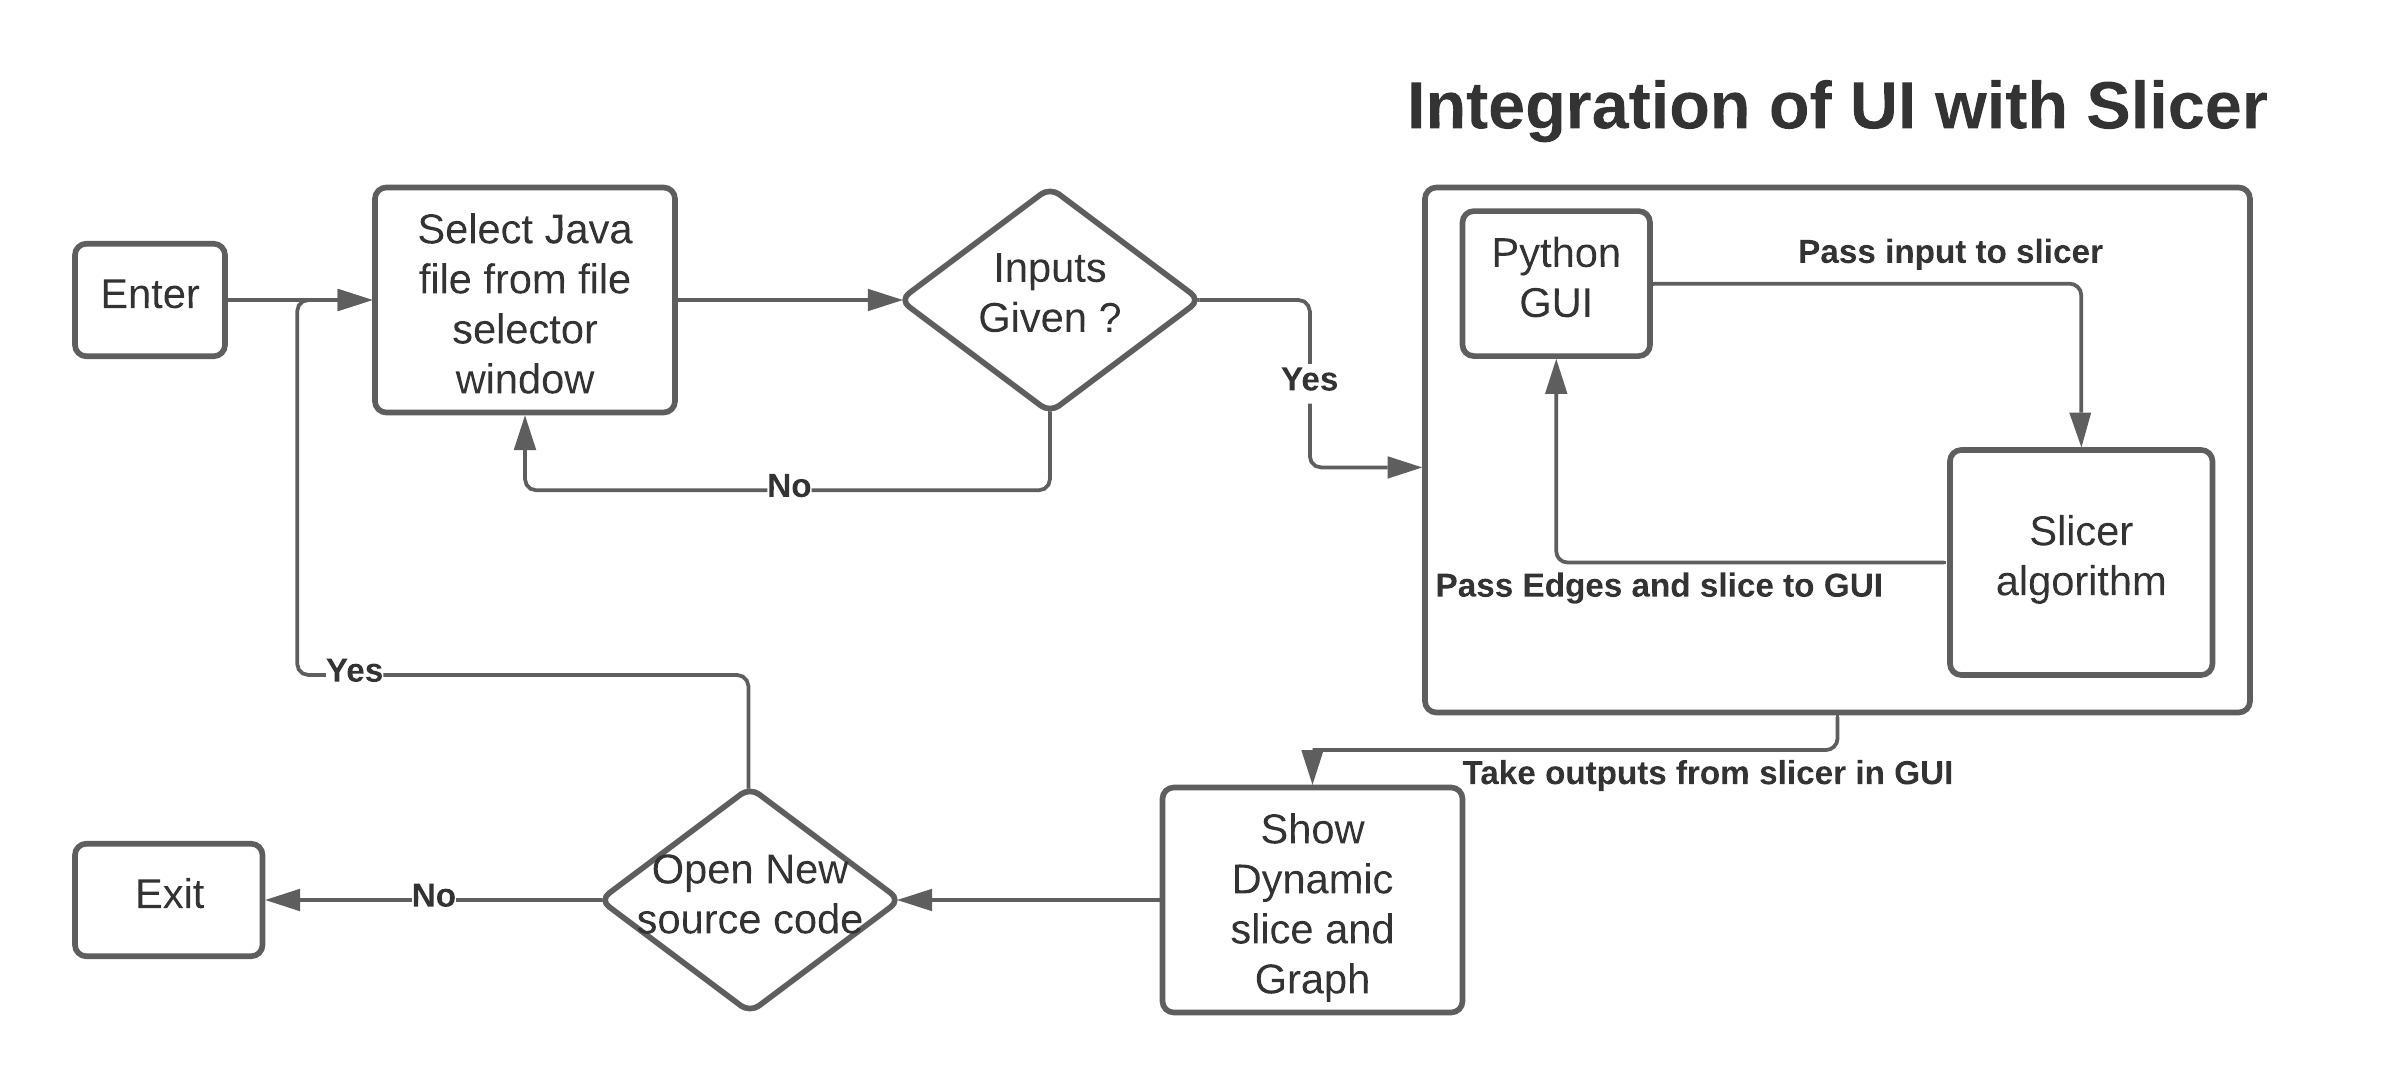
\includegraphics[scale=0.4]{Blank diagram (1).jpeg}\\
\subsection{Block diagram}
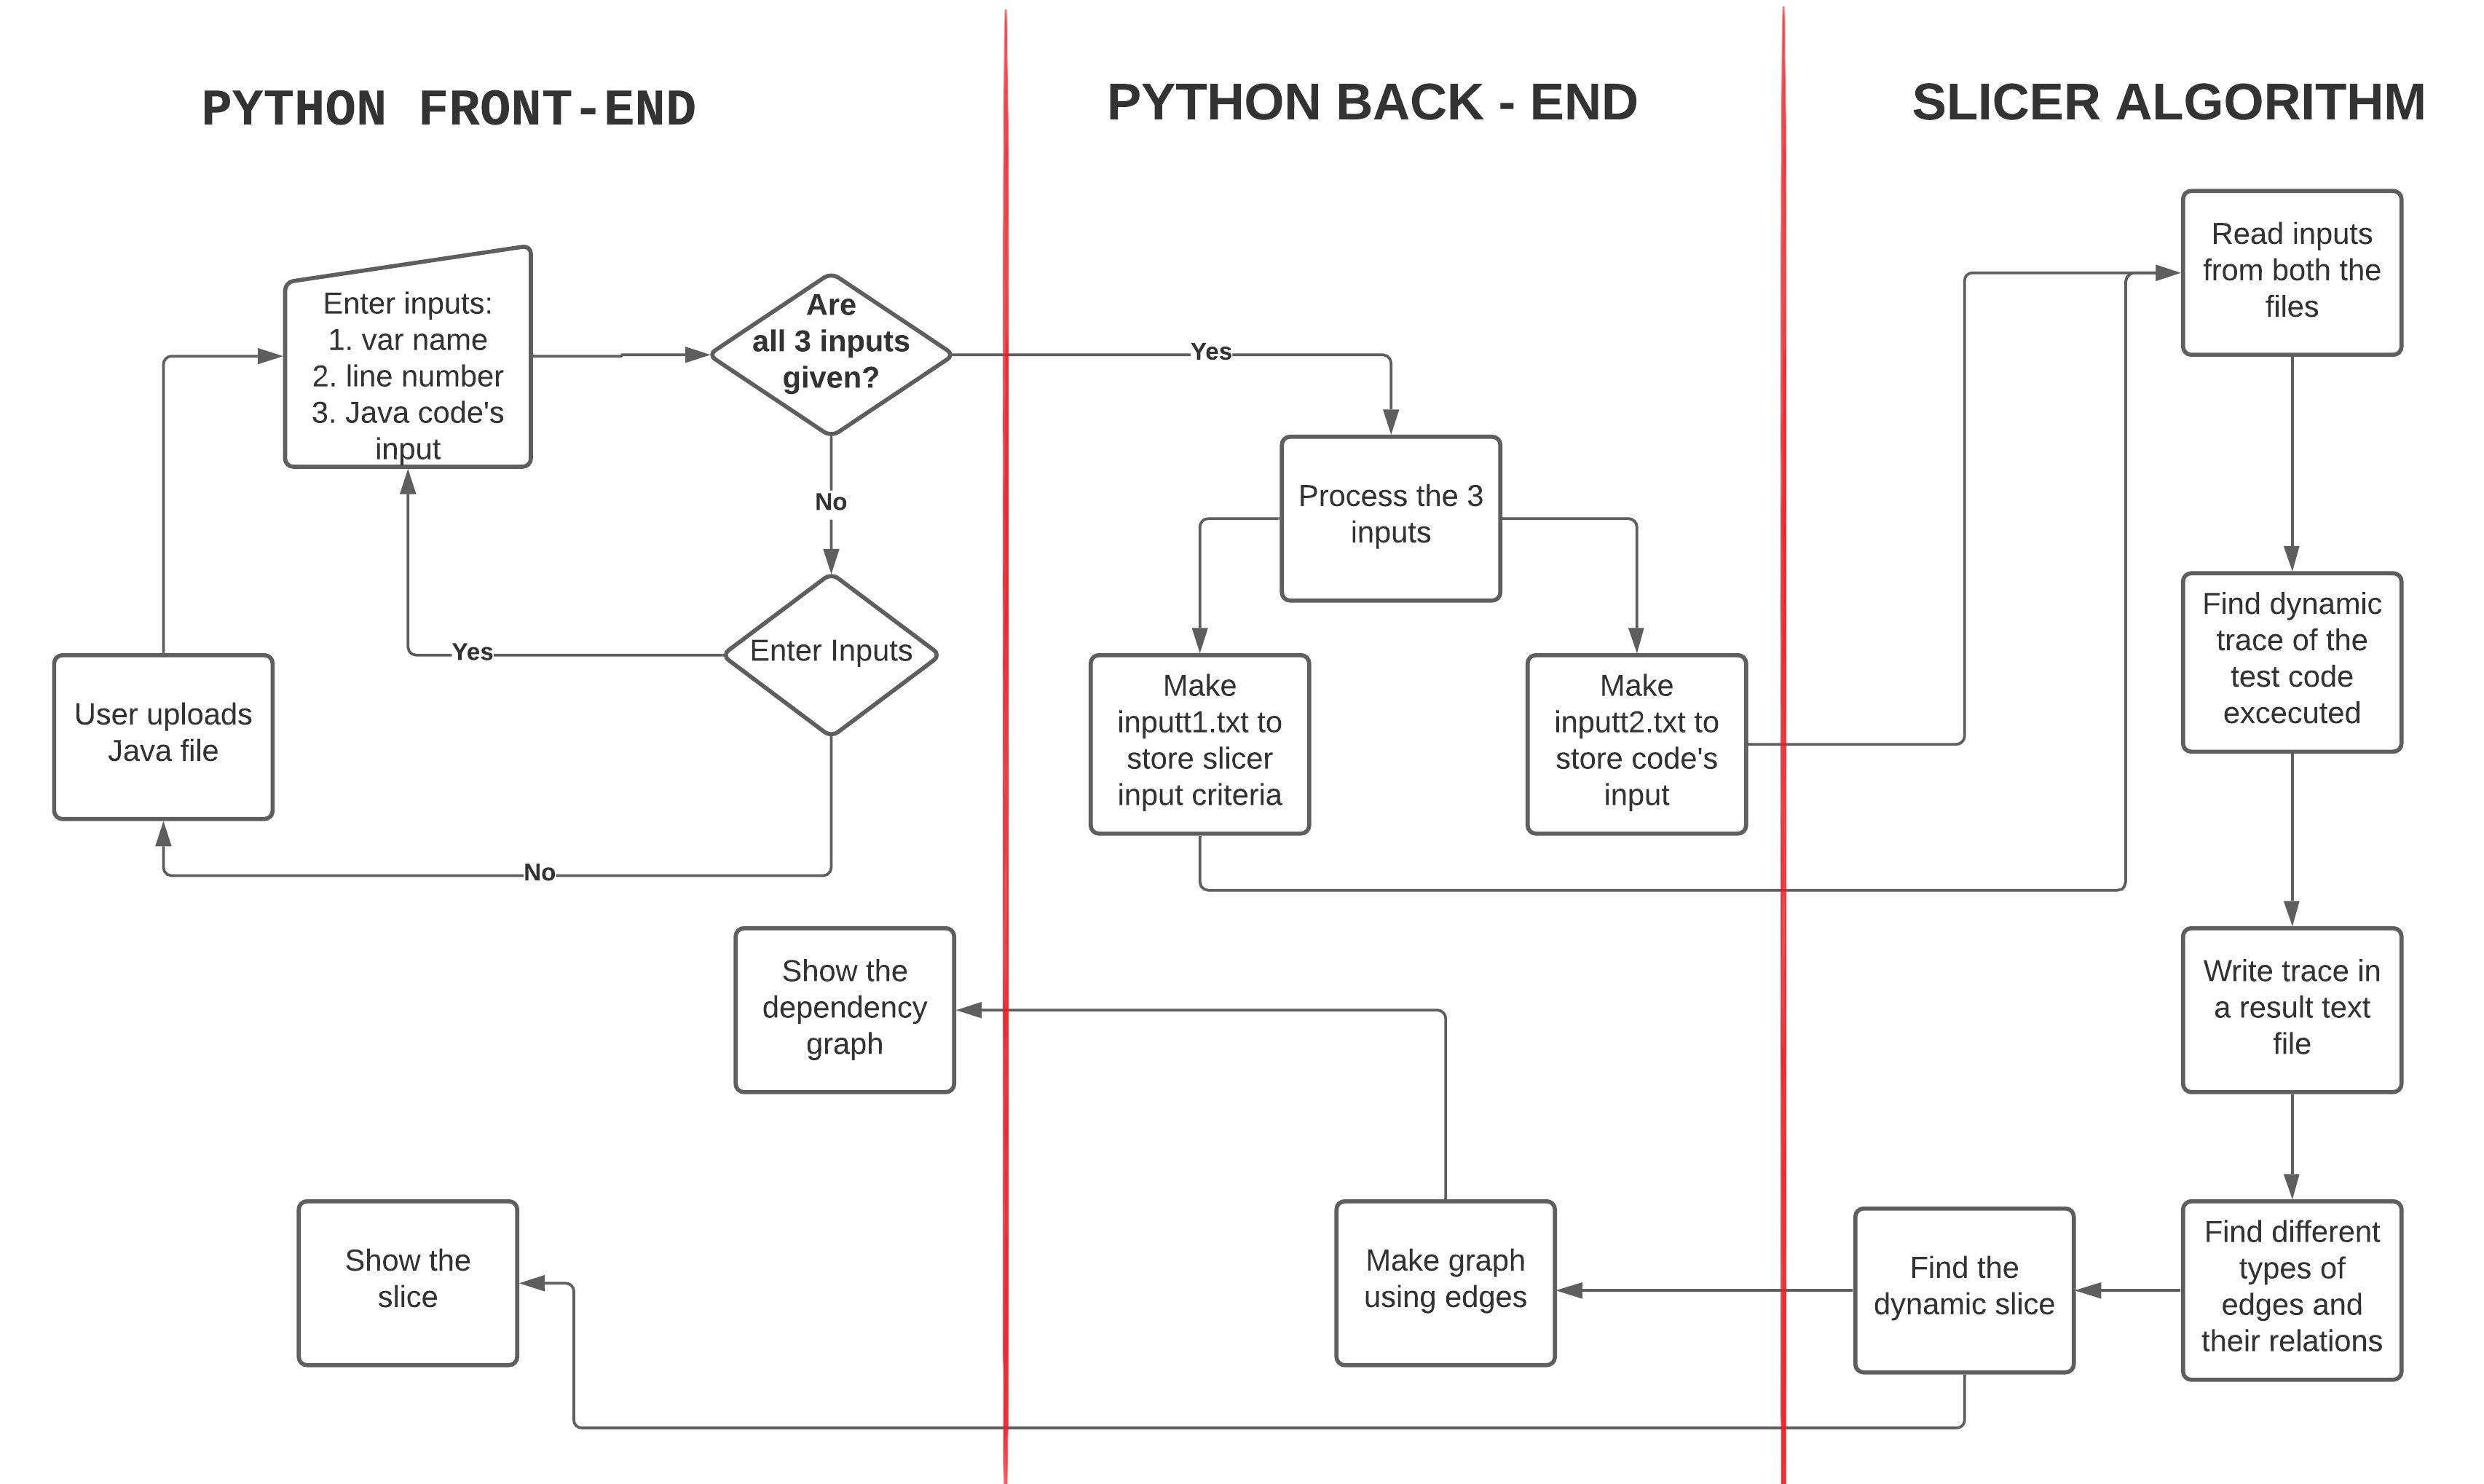
\includegraphics[scale=0.3]{Blockkk.jpeg}
\subsection{Logic}
The main logic of implementation starts when user uploads Java source code and the algorithm takes the source code and modifies the source code which will be needed to trace back the lines which will be executed in terms of dynamic slicing. After this process is done the algorithm executes the updated source code only if system supports the Java i.e. Java compiler is a prerequisite else the algorithm stops. Since in order to calculate the dynamic slice, there is a need that algorithm should first go through the whole source code and so the next step is to parse source code starting from first line.Moreover, Since this is an algorithm of Dynamic slicing, there is a need of system input to the source code because depending upon the system inputs some instructions of code may or may not get executed. Like, if there are conditional statements in the code, then either if or else if part of the program will get executed. So on the basis of system inputs and instructions the algorithm will create different vertexes and different kinds of edges between dependent vertexes based upon the relations between them. When the parsing of code till slicing line number is completed then the next step of algorithm is to create a SDG, so that algorithm can start slicing on this graph.

The user needs to input 3 things in order to execute a slicer:
\begin{itemize}
    \item Source code of Java program
    \item Slicing criterion 
    \item User inputs to the variables
\end{itemize}

When the algorithm is parsing the code,it will only parse the code till the slicing criteria mentioned in the input. While parsing the code, the algorithm stores different kind of dependencies between the statements. The algorithm generates SDG which has:
\begin{itemize}
    \item Nodes: Instructions in the source code. Remember, for the simplicity of the algorithm, we kept only one instruction per basic block
    \item Edges: Different types of dependencies between the nodes
\end{itemize}

Some additional nodes need to be created in order to handle functional calls. These nodes are based on the way function or method is declared and called. The four additional types of nodes required for handling functional calls are as below:
\begin{enumerate}
    \item Actual in-nodes:for all function arguments
    \item Actual out-nodes : for the function arguments (passed by reference)
    \item Formal in-nodes : at called procedure node for all function parameter
\item  Formal out-nodes : for the function parameters passed by reference
\end{enumerate}

To understand slicing of functional calls in a better way, consider the below example:
\verbatiminput{eg.txt}
The different types of nodes created are as follows:
\begin{itemize}
    \item Actual out nodes: a=x\textunderscore out, b=y\textunderscore out
    \item Formal out nodes: x\textunderscore out=x, y\textunderscore out=y
    \item Actual in nodes: a\textunderscore in=a, b\textunderscore in=b
    \item Formal in nodes: x=a\textunderscore in, y=b\textunderscore in
\end{itemize}

The different type of dependency edges required to capture all the dependencies are as follows:
\begin{enumerate}
    \item Control Dependence Edge : Edge from node A to node B states that execution of node B is controlled by node A
    \item Data Dependence Edge : Edge from node A to node B with respect to some variable v states that value of v in node B is transmitted by node A
    \item Parameter-in Edge : Edge between actual-in and formal-in nodes, representing the functional call
    \item Parameter-in Edge : Edge between actual-out and formal-out nodes, representing the functional call
    \item Transitive Dependence : This edge links between actual-out and actual-in nodes
    \item Affect-return Edge : This edge is created between the call node X present in call site which is expecting a return value and the actual-in node
    \item Call Edge : A call edge is to a caller X from a call site node Y
\end{enumerate}
The algorithm tries to approach this slicing problem in two passes. However, 
in terms of computer vocabulary we can classify this algorithm under the topic of reachability of graphs. This approach can be viewed as modified version of DFS. During the first phase of the traversal, the slicing algorithm just as in DFS visits and then marks different nodes that are directly or indirectly or transitively connected to the node N of the slicing criteria as well as procedure Q of the slicing criteria or to the procedures that directly or indirectly or transitively calls the procedure Q. Just as in DFS, the algorithm reaches up till its maximum height (or reaches down till its maximum depth) and then iterates up, this algorithm behaves the same way and traverses up and never traverses down into the called procedure Q.

The algorithm that runs slicer operates with different types of edges as shown
above, however data dependence edge and control dependence edge are being
added only till the scope of the variable i.e. where it was last defined or where it was last used or the node and its enclosing node.

The whole logic can be summarized in a very simple manner. The first phase of the algorithm remembers and keeps the track of the nodes visited while traversing upwards and during the second pass all the types
of edges given above are considered and system dependence graph is constructed. The last part of the algorithm merges the nodes from each phase to get the final state of SDG obtained from the slice. And hence, the algorithm terminates when it reaches the line number mentioned in the slicing criteria and gives the relevant set of nodes affecting that particular line.
\subsection{Pseudocode}
Input: P : a program

Output: System Dependence Graph for P
\begin{enumerate}
    \item Go through the source code line by line and parse the lines and depending upon different keywords create different vertices for each line
    \item Store defined and used variables on that line in that line’s vertex
    \item Create Data dependence edge from used variable’s vertex to where that used variable is last defined before the used variable’s line
\item Create Control dependence edge from current vertex to its enclosing scope vertex
\item On the procedure definition line, create formal-in vertices for all procedure parameters, formal-out vertices for all procedure parameters which are passed by reference and procedure vertex
\item On the procedure call line create call site vertex, actual-in vertices for all procedure arguments and actual-out vertices for all procedure arguments which are passed by reference
\item Create a call edge from the call site vertex to its corresponding procedure vertex
\item Create parameter-in edge for all actual-in vertex at call site between actual-in vertex to its corresponding formal-in vertex
\item	Create parameter-out edge for all formal-out vertex between formal-out vertex to its corresponding actual-out vertex
\item	If there exist intraslice-path from the formal-out vertex to formal-in vertex then create transitive dependence edge from an actual-in vertex to an actual-out vertex 
\item If there exist intraslice-path from the formal-out vertex to formal-in vertex then create affect-return edge from an actual-in vertex to the call site vertex 
\item Create return-link edge for each return site in the called procedure Q from the return vertex in Q to each call site vertex that calls Q
\end{enumerate}
The slicer works in two phases. The phases are described below in the pseudocode :
\begin{enumerate}
    	\item Take the source code and augment it by adding lines to get the execution trace and than compile that augmented source code
\item	Go through the execution trace generated in above step and call construct\textunderscore SDG function by passing current executed source line
\item	Repeat the above step until there are lines left in the execution trace
\item	Now process the generated graph from the above steps in 2 phases
\item	Phase1
\begin{itemize}
\item	Push the slicing vertex in the queue
\item	Now repeat below steps till queue is not empty
\item	Push the queue’s front vertex’s parent, parameter in edge, calling edge, transitive edge, and affect return edge in the back of the queue
\item	Pop the first element of queue
\end{itemize}
\item	Phase 2
\begin{itemize}
\item	Push all the visited vertex till this point in the queue
\item	Now repeat below steps till queue is not empty
\item	Push the queue’s front vertex’s parent, parameter out edge, return link edge, transitive edge, and affect return edge in the back of the queue
\item	Pop the first element of queue
\end{itemize}
\item Return all the visited vertices
\end{enumerate}

\subsection{Implementation}
The algorithm for the slicer has been implemented in C++. The following is the step wise implementation of the algorithm:
\begin{enumerate}
    \item When the user executes the slicer code, the slicer code uses system call named system() to execute the java source code. The java source code should be named as source.java and should contain only one class named source. 
    \item Now, the slicer parses the source code and dynamically adds few lines to original source code and created a new code in file named "Outputnn.java". The new lines are written above each line of original source code with sole purpose of redirecting the line numbers to the new text file. While parsing this file, dependencies are stored with the help of data structures, which would help in creating system dependence graph
    \item This file starts getting executed and creates a new file named "resultt.txt" which contains the line numbers of the statements that got executed.
    \item The slicer runs the modified version of graph reachability algorithm (BFS) in order to find the dynamic slice of the variable of interest at particular line number. The dynamic slice is calculated on the basis of dependencies between the line numbers. An array is maintained which maps line numbers to the instructions. With the help of this array, the actual dynamic slice is obtained.
    \item The final step of the slicer is to create different files for different types of dependencies. This is so that system dependence graph can be created and visualized. 
\end{enumerate}
All the files mentioned above are automatically deleted by the code itself once the system dependence graph has been created. Several containers and data structures need to be maintained. They are as follows:
\begin{itemize}
    \item A map mapping line numbers to their nodes in the graph
    \item A container to store all the definition nodes of the variables
    \item A container to store all the function nodes
    \item A container to store all the return statements
    \item A list of inbuilt datatypes that the slicer will be able to handle
    \item A stack for maintaining scope of variables
    \item A stack for evaluating control dependencies
    \item An array to map line number to their respective instructions
    \item An array to store the hierarchy of conditional statements
\end{itemize}
\subsection{Integrating back-end with GUI}
\begin{itemize}
\item For designing of GUI, we have used Tkinter, it is basically a Python binding to the Tk GUI toolkit and is a stadard GUI tooklit in Python. There are 3 files needed for the implementation which are as follows:
\begin{itemize}
    \item Source code (Java file)
    \item Slicer (C++ implementation)
    \item Python GUI (Using Tkinter)
\end{itemize}
\vspace{0.5 cm}
\item On running the GUI, it launches a dialogue box which first checks if Java compiler is installed in the system or not, if it is not installed then the slicer cant be functional, hence it reaches at the dead-end. However, if Java compiler is available in the system then on clicking the "Select File" button, the user will be given the choice to select any Java file from the system and on selecting the file a new window frame is invoked which gives the code preview of the file selected and options to write variable name and standard inputs.\\


\vspace{0.25 cm}
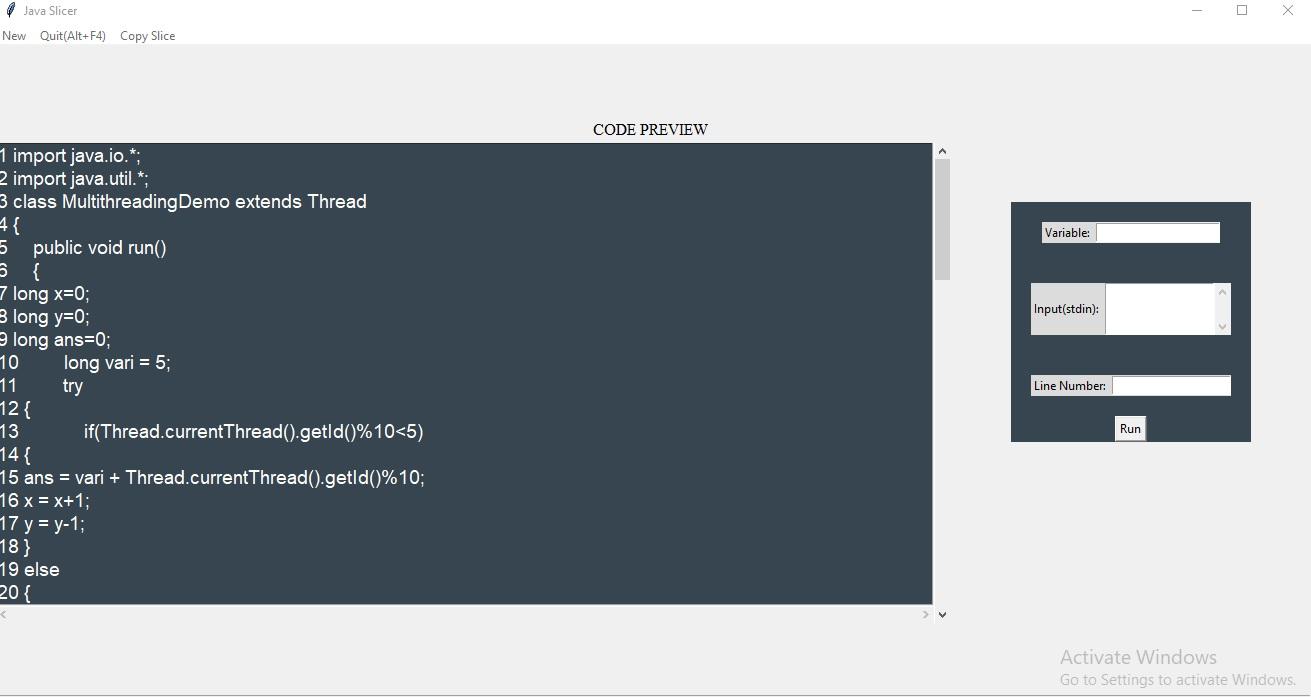
\includegraphics[scale=0.2]{UI_1.jpg}\\
\vspace{0.5 cm}
\item Select the line for which we want to compute the slice and writing the variable name for dynamic slicing along with the "stdin"\\


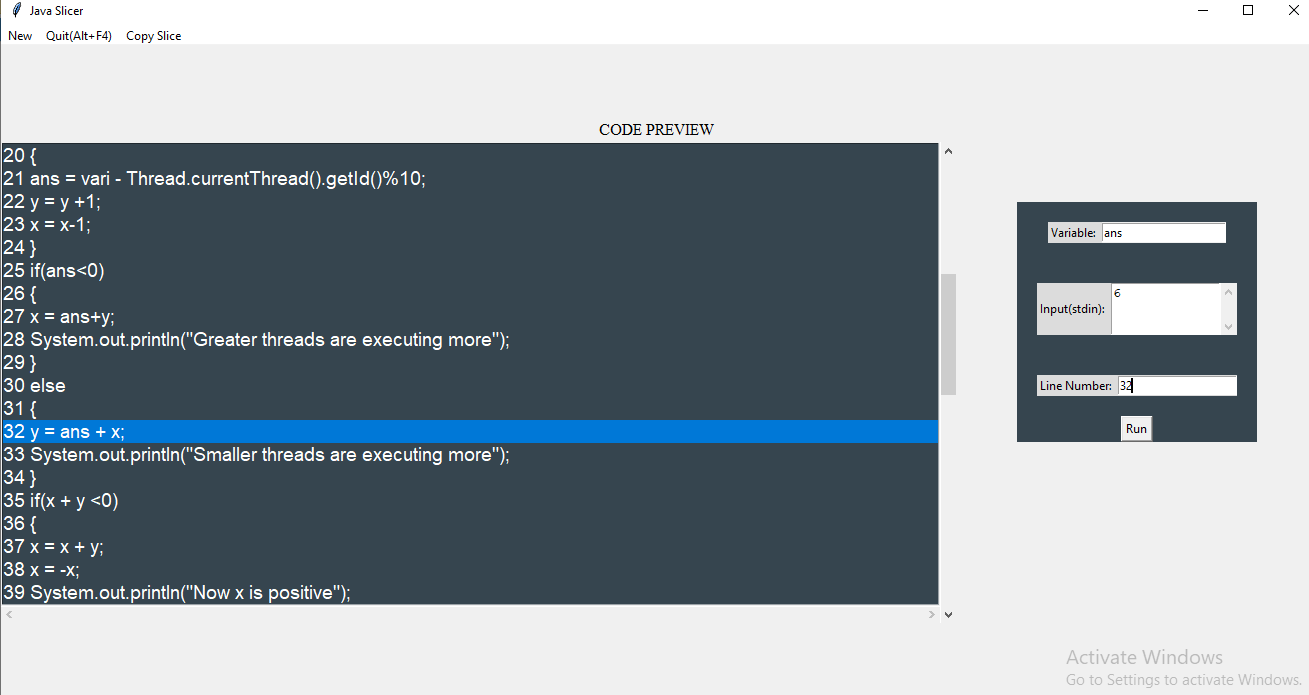
\includegraphics[scale=0.2]{UI_2.png}\\


\item The slicer running in the back-end of the GUI will give two output windows:
\begin{itemize}
\newpage
    \item Dynamic slice\\
    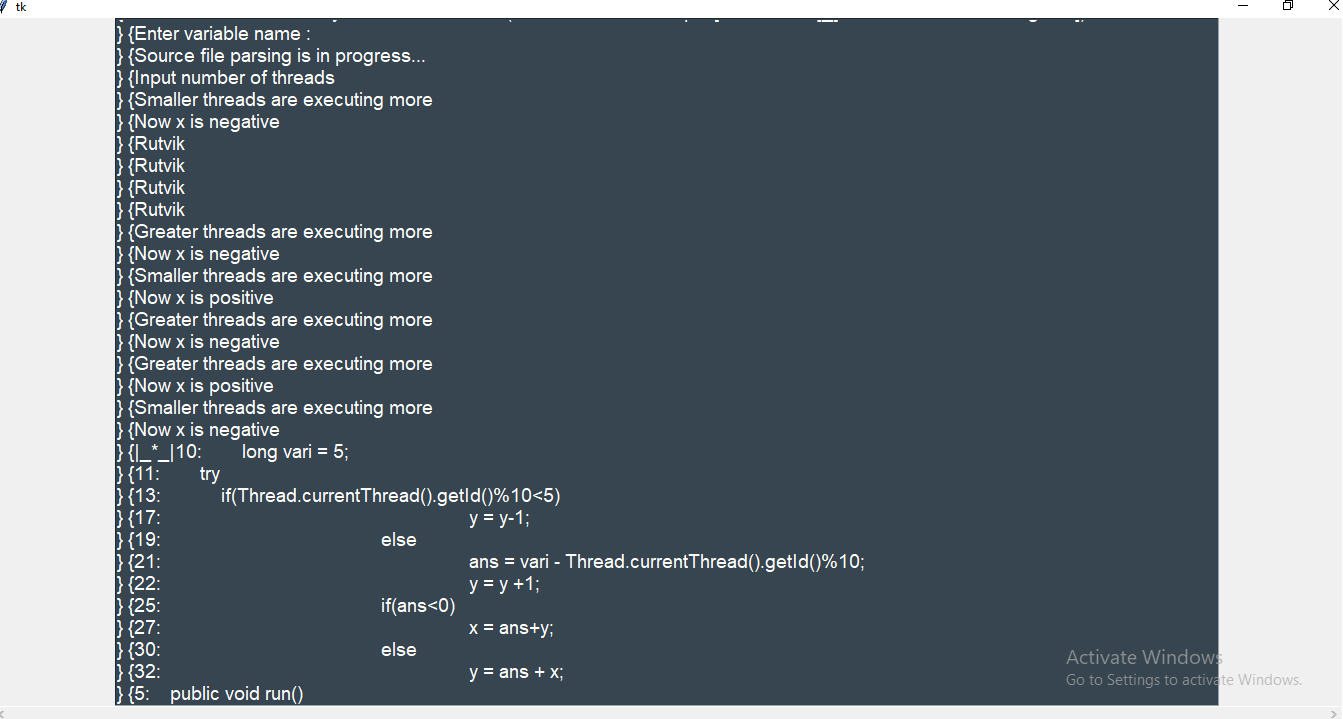
\includegraphics[scale=0.2]{UI_3.png}
    The above image shows an example of output window of dynamic slice obtained after running the dynamic slicer on one of the examples mentioned in this report.
    \item Dependency Graph: Dependency graph is created from the different files that were created when the slicer executed the source code. For visualizing graph, we have used networkx library of python to create a directed graph. The graph uses different colours for edges of different dependencies so that dependencies can be visualized properly from it.
    
    \begin{flushleft}
    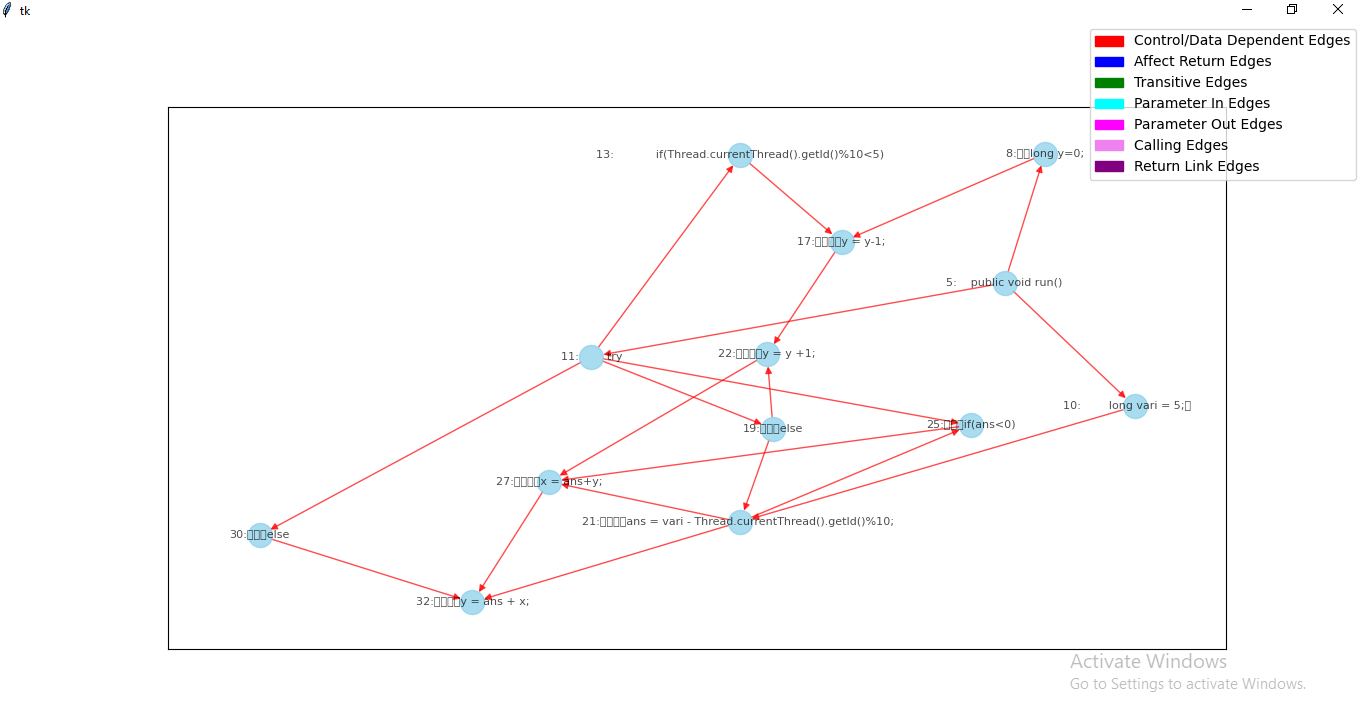
\includegraphics[scale=0.25]{UI_4.png}
    
    \end{flushleft}
    
\end{itemize}
\end{itemize}
\begin{itemize}
    \item  Also, there is an option available named "Copy Slice" which copies the output slice to clipboard.
\end{itemize}

\section{Example of Simple Java functionalities}
\subsection{Source Code}
\verbatiminput{source_orig.java}
\subsection{Slice Criterion}
\begin{flushleft}
Input var : y\\
Input line : 42\\
Code Input  :\\
1\\
2\\
3\\
4\\
\end{flushleft}
\subsection{Slice and Dependency graph}
\verbatiminput{out1.txt}
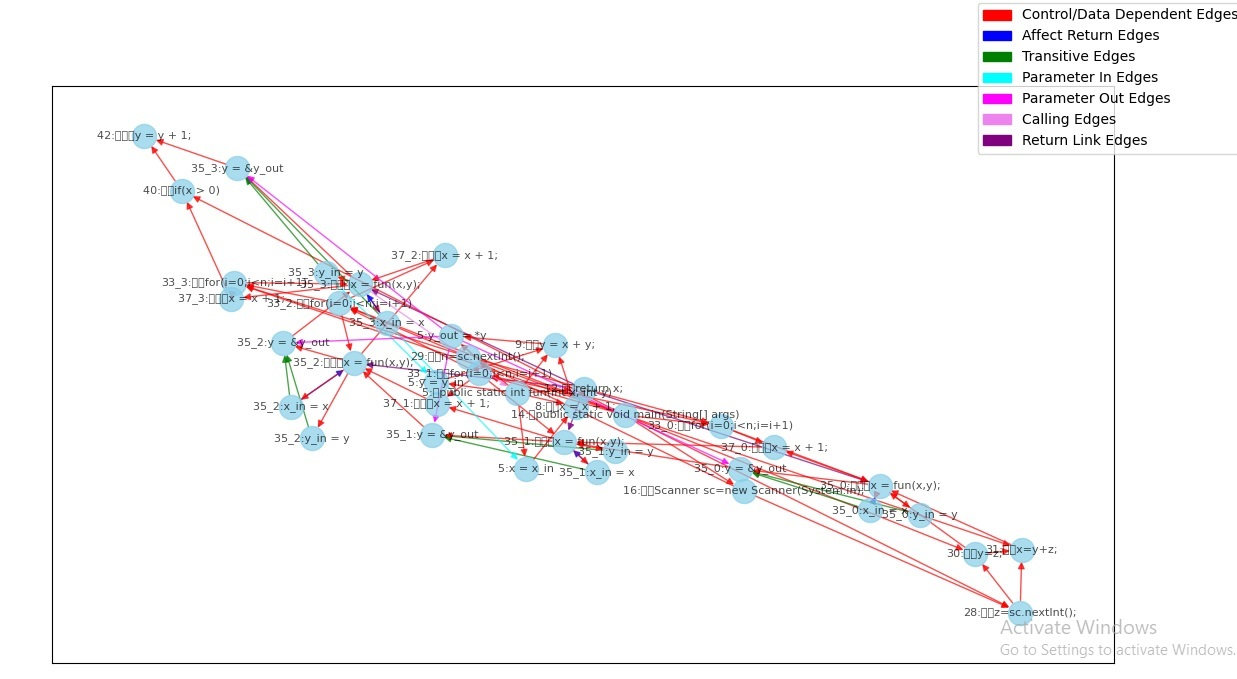
\includegraphics[scale=0.3]{G1.jpg}
\subsection{Explanation}
\begin{itemize}
    \item Since this is an algorithm for dynamic slicing, the output would only contain instructions that were actually executed after the user input. Since we chose line number to be 42, the statements before the line number would only be considered. Now execution of line number 42 is control dependent on line number 40 i.e. will depend on the value of x.
\item Now, the statement on line 40 is data dependent on line number 37. The value of x on line number 37 is data dependent on the value of x obtained on line number 35.

\item The execution of line number 35 is dependent on line number 33. Hence, there is control dependency between line number 33 and 35. Thus, the execution of line number 35 is dependent on the value of n.

\item The instruction on line number 35 is data dependent on the value of x obtained on line number 31. which is in turn is data dependent on line number 30 for value of variable 'y'. The value of y on line number 30 is data dependent on value of 'z' on line number 28 that is being scanned. The for loop on line number 33 is data dependent on value of 'n' and hence is data dependent on line number 29.
\item Also,  the value of 'x' at line number 35 is dependent on the value that the function fun(x,y) returns.
\item The statements y\textunderscore in=y and x\textunderscore in in output slice represent the actual in nodes ans the statement y=\&y\textunderscore out represent the actual out nodes as explained earlier in the logic section. 
\item The line numbers like 33\textunderscore 0 present in the output slice represents the first iteration of loop at line number 33. 

\end{itemize}

\section{Example of Threaded Java program}
\subsection{Source Code}
\verbatiminput{2.txt}
\subsection{Slice Criterion}
\begin{flushleft}
Input var : y\\
Input line : 43\\
Code Input  :\\
8
\end{flushleft}

\subsection{Slice and Dependency graph}
\verbatiminput{out2.txt}
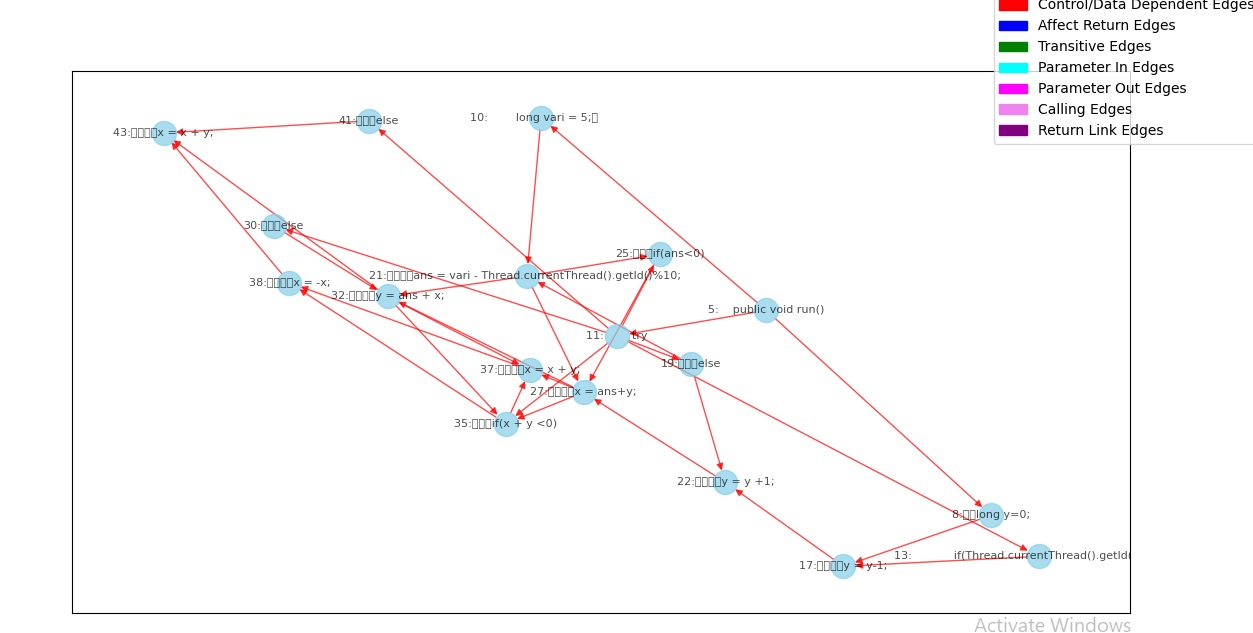
\includegraphics[scale=0.25]{G2.jpg}
\subsection{Explanation}
\begin{itemize}
    \item The execution of statement on line number 43 is dependent on the values of x and y in the conditional statement on line number 35.
    \item The values of x and y depends on the value of ans due to conditional statement present on line number 25.
    \item The value of x on line number 43 is data dependent on statement on line number 22.
    \item The value of ans on line number 25 depends on statement on line number 21. There is data dependence between both the statements.
    \item The execution of line number 21 depends upon the execution of line number 13 which means there is control dependency between line 13 and line 21
    \item The value of ans variable on line number 15 depends on the value of variable "vari" which is defined on line number 5 and hence there is data dependency between line number 5 and line number 13.
    \item Line number 13 executes only when try block gets executed and hence there is control dependency between line number 13 and line number 11
\end{itemize}
\section{Testing}
We started adding functionalities to the slicer one by one and tested the previous functionality before adding the new one. The testing was done manually. We first added the support for datatypes and scanner class in our slicer and tested it for various user inputs as well as different slice criteria for different programs. After implementing the basic functionalities, we tested it on several programs and then the support for API and functional calls were added. The above mentioned examples are some of the source codes that we used, after the slicer was ready, when we tested at the final stage. 
\section{Future Work}
As mentioned earlier, Java is quite a large language and hence Java has so many functionalities that can be added. The slicer will become more and more useful as support for additional functionalities are added. Some of the functionalities that can be added is support for object oriented concepts like inheritance, abstract classes, polymorphism etc. Also, functionalities such as JDBC can also be added so that the dynamic slicer becomes more useful to the developers out there.

The another part that can be added to the slicer is implementing a static slicer for the same functionalities and test both static and dynamic slicers for same program and compare the efficiencies of both the slicers. Efficiency means comparing number of instructions in the program slice. Also, graphless algorithms can be implemented and similarly efficiency comparison can be done. 
\section{Conclusions}
The project developed a tool for calculating dynamic slicing for Java programs. An algorithm for dynamic slicer was implemented and some of the functionalities of the Java code were added. The tool also shows dependency graph which can be helpful to the user in visualizing the slice in a better way. The Dynamic slicer would help a user in debugging as well as testing programs.    
\section*{Acknowledgment}
\begin{itemize}
\item We would like to express our humble gratitude to our BTP Guide and supervisor, Jayprakash Lalchandani sir, who guided us throughout this project. One of the major important skill apart from technical knowledge and implementation logic that we learnt from our Prof. Jayprakash Lalchandani sir was to know how to interpret the Research papers and implement them along with precise time management and we are highly obliged to him to provide us with such a fascinating topic.
\item We would also like to thank our university DA-IICT to provide us with this invaluable opportunity of Btech project and all the faculty members who are immensely trying to aid us to successfully achieve the target of our BTech project. Last, but not the east we would like to thank our fellow batch-mates, family members and the almighty for the extensive support.  
\end{itemize}    
\begin{thebibliography}{00}
\bibitem{b1} Hiralal Agrawal,Department of Computer Sciences,Purdue University,West Lafayette, IN 47907-2004 and Joseph R. Horgan,Bell Communications Research,Morristown, NJ 07960-1910, Title : Dynamic Program Slicing
\bibitem{b2} FRANK TIP*, IBM T.J. Watson Research Center, PO Box 704, Yorktown Heights, NY 10598, USA, Title : A survey of Program Slicing Techniques
\bibitem{b3} Matthew Bridges, Title : Program Slicing of Explicitly Parallel Programs
\end{thebibliography}
\vspace{12pt}

\end{document}
